\chapter{Conclusions}
\label{chap:conclusions}

\section{Summary of Results}
%Intro/recap
Studies of the \Hgg decay have been carried out using both a BDT-based VBF tag and a DCNN-based VBF tag with 35.9\,fb$^{-1}$ of $\sqrt{s}=13$\,TeV data. 
The Higgs boson is observed with high significance and measurements made of signal strength and coupling modifiers. 
These measurements are summarised in Table \ref{tab:conclusion:measurements}.
\begin{table}[h!]
    \centering
    \renewcommand{\arraystretch}{1.5}
    \begin{tabular}{ l | c c c c}
        \thickhline
        Measurement & \multicolumn{2}{c}{BDT-based VBF}  & \multicolumn{2}{c}{DCNN-based VBF} \\
        \hline
        $\mu$ (Global)                  & \multicolumn{2}{c}{$1.18^{+0.17}_{-0.14}$} & \multicolumn{2}{c}{$1.23^{+0.16}_{-0.15}$} \\
        $\mu_{\mathrm{VBF}} $           & \multicolumn{2}{c}{$0.8^{+0.6}_{-0.5}$} & \multicolumn{2}{c}{$1.5^{+0.5}_{-0.4}$} \\
        $\sigma^{\mathrm{VBF}}_{proc}/\sigma^{\mathrm{VBF}}_{theo}$ & \multicolumn{2}{c}{$0.8^{+0.6}_{-0.5}$} & \multicolumn{2}{c}{$1.4^{+0.5}_{-0.4}$} \\  
        $\mu_F$, $\mu_B$                & $1.19^{+0.22}_{-0.18}$ & $1.21^{+0.58}_{-0.51}$ & $1.xx^{+0.xx}_{-0.xx}$ & $1.xx^{+0.xx}_{-0.xx}$ \\
        $\kappa_F$, $\kappa_B$          & $1.xx^{+0.xx}_{-0.xx}$ & $1.xx^{+0.xx}_{-0.xx}$ & $1.xx^{+0.xx}_{-0.xx}$ & $1.xx^{+0.xx}_{-0.xx}$ \\ 
        $\kappa_{\gamma}$, $\kappa_{g}$ & $1.xx^{+0.xx}_{-0.xx}$ & $1.xx^{+0.xx}_{-0.xx}$ & $1.xx^{+0.xx}_{-0.xx}$ & $1.xx^{+0.xx}_{-0.xx}$ \\ 
        \thickhline
\end{tabular}
    \caption{Measurement results.}
    \label{tab:conclusion:measurements}
\end{table}


%DCNN
The DCNN-based measurements have demonstrated significant improvement over the BDT-based approach \cite{HIG-16-040} used since the Higgs boson was discovered \cite{CMS_Higgs_disc}.
Expected significance and purity in the VBF tag are improved leading to reduced uncertainty on the measurements, particularly those affected by the VBF tag. 
For this to be achieved the training had to be split into two steps: one for feature learning from the jet images, and one for the actual classification problem with the costs defined appropriately.
Furthermore, the unique problems posed by the sparse nature of the jet images also required particular training conditions. 
Gradient clipping regularisation was needed to control large parameter updates early in the training, and an adaptive optimiser was needed to handle how the sparseness affects the frequency of parameter updates.

The DCNN learns to construct physically sensible and robust features from correlations in structure between the jets.
This was shown by data-simulation validation on \Zee, and by evaluating how the network performs over different modelling variations. 
The features themselves were extracted using feature visualisation to produce maximally-activating images for the class logits (and at other point in the network in Appendix \ref{appendix:feature_vis}). 
These features were found to correspond to expected properties of VBF and ggH production, a particular example of this being the distortion of the jets by colour connection in VBF.

The DCNN-based measurements along with the validation and interpretation demonstrates that the DCNN-based VBF tag is superior and DCNNs have great potential in particle physics analyses.
However, this is still a relatively new technology in the field of particle physics and will need to be studied closely for its precise systematic effects.




\section{Future Development}
The most immediate future improvement could be the application of a similar DCNN to VH hadronic signal extraction.
This is currently achieved using a set of kinematic cuts and could be improved with a ML based approach.
When the associated vector boson decays hadronically there will be structure correlations from colour connection in the resulting dijet and characteristic charge deposition.
These are features a DCNN could pick up on.

In 2026 the LHC will have been upgraded to the High-luminosity LHC (HL-LHC) \cite{HLLHC} to provide much higher instantaneous luminosity resulting in a substantially larger dataset. 
This collision environment will pose particular challenges for the CMS detector's hardware and operation, as well as CMS analyses.  
Pileup will increase to 200 collisions per event and radiation dose to the detector itself will be markedly increased. This has necessitated the future replacement of the CMS endcap calorimetry by a high-granularity silicon sampling calorimeter with many readout channels \cite{HGC}. 
The difficulty of extracting physics objects in such an environment, and in accurately reconstructing them from such high-dimensional data, may be areas where deep learning approaches will prove to be especially important. \\


There are many avenues to investigate for the development of future ML algorithms and where to apply them. 
A few possible directions are outlined here: neural attention, generative adversarial networks (GANs), and ML algorithms more suited to the natural structure of jets.

Neural attention \cite{Attention,SpatialTransformer} inserts a mechanism that allows the network to transform and focus on particular parts of the input depending on what features are present. 
This facilitates the construction of long-range dependencies between different input regions, for example different parts of an image.
This could be useful in processing jet images by picking out dependencies between clusters of PF candidates in the jet more efficiently.
However, given the non-standard behaviour of the polar jet images the way the transformations are applied will need to be handled carefully to be compatible with the periodic boundary condition.

GANs \cite{GANs} are generative models that attempt to model the underlying data-generating process $P(\vec{x})$ itself and can achieve remarkable results (Figure \ref{fig:conclusion:progan}).
\begin{figure}[h!]
    \begin{center}
        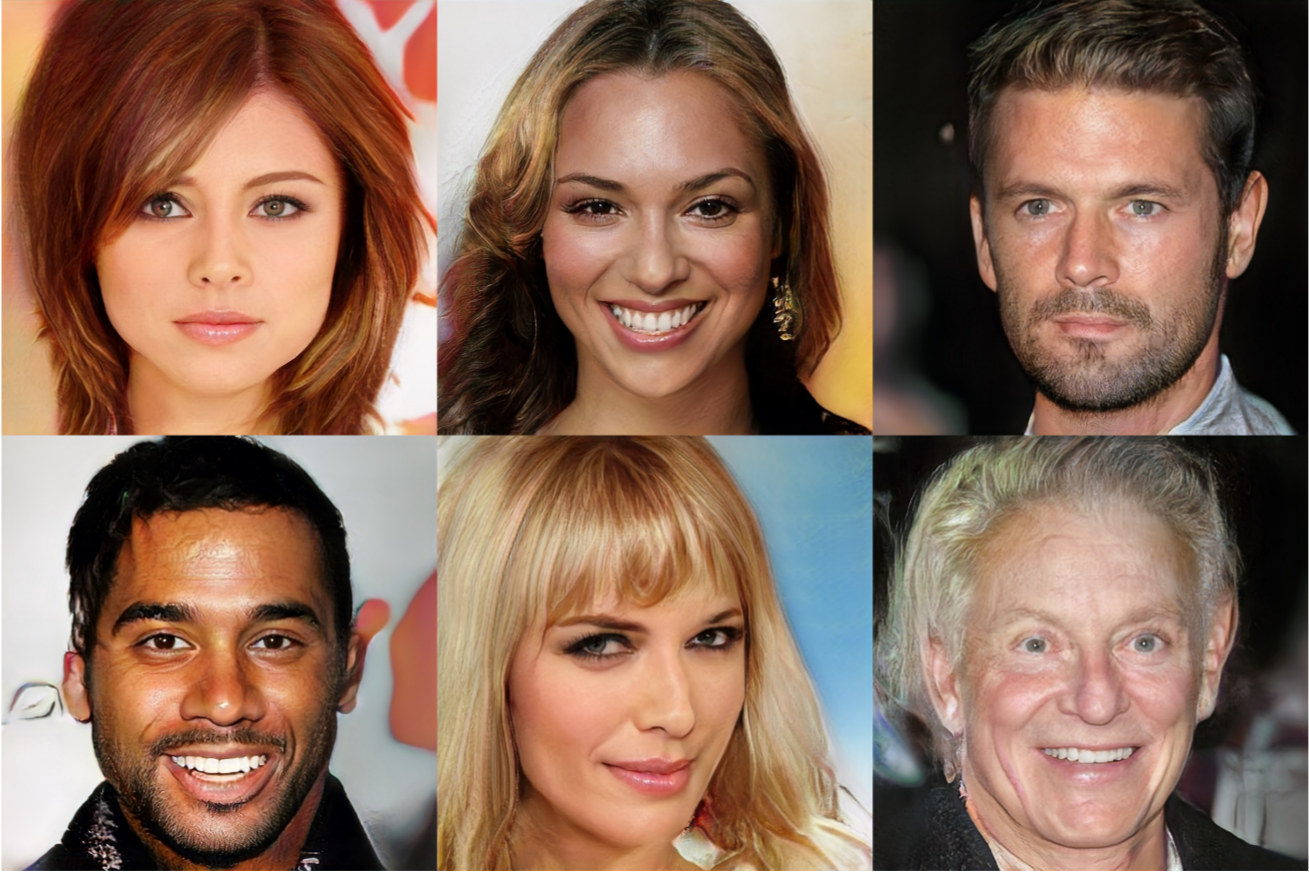
\includegraphics[width=0.8\textwidth]{figures/conclusion/progan.png}
    \end{center}
    \caption{Fake celebrity faces generated by a progressive GAN \cite{ProGAN}.}
        \label{fig:conclusion:progan}
\end{figure}

These consist of two competing networks: the generator and discriminator. 
The generator makes `fake' examples given a vector in a space, and the discriminator tries to tell these fake examples from real ones. 
During training each learns from the other and once fully trained the generator ideally becomes a realistic generative model, and the discriminator develops many useful discriminating features.

Both the generator and discriminator may have application in particle physics analyses. The generator could be used to enhance under-populated samples to improve cut optimisation or ML model trainings (an example may be found in \cite{GANChest}).
The discriminator could be used to learn features from data that can then be used in another training, this was shown to work well in \cite{DCGAN}. 
In a physics analysis this could be achieved by training a GAN on real data with a CNN as the discriminator, then using the frozen convolutional layers of the discriminator in another training over simulation. 
This would be like the two step training of the VBF DCNN model but with the discriminator features used instead of step one.


Finally, the components and structure of CNNs are geared towards images with locality and translational invariance in their features that can then be combined hierarchically. 
Recurrent neural networks (RNNs) make similar assumptions over a sequence. 
However, jets are not naturally images or lists. They have a tree structure where an initial parton gives rise to multiple daughter particles that then fragment or decay to more daughter particles.

The assumptions in an ML algorithm's construction determine how it makes predictions and is referred to as its `inductive bias' \cite{InductiveBias}.
The polar jet image formulation was a way of representing jets in a way that works with the inductive bias of CNNs, but it may be better to use an algorithm that is suited to trees or graphs.
Examples of such algorithms are recursive neural networks (Chapter 10 of \cite{DeepLearningBook}) that extend the sequence processing of RNNs to tree structures, and graph CNNs \cite{GraphCNNs} that have analogues for convolution and pooling given graph-based input.


\section{Conclusions}
All of these measurements are compatible with predicted values for a Standard Model Higgs boson, but there is ample room for deviation within uncertainty.
This uncertainty will be reduced as the available dataset increases in size over the Run II era and onwards. 
As the measurements become less dominated by statistical uncertainty systematic uncertainties in precision measurements will become especially important, in particular contamination of categories such as VBF by ggH. 
Here the DCNN approach will be especially useful for constructing high-purity samples when overall significance is less of a priority.

The fields of Higgs physics and machine learning have now entered a new era of scale, precision and sophistication.
Hopefully BSM signals are hidden within the uncertainties of our measurements and ML will will grant us the power to extract them as our dataset expands.
There is a bright future for both fields with great potential for collaboration between them and lots of work to be done. 









